\subsection{Datasets}
\begin{frame}
  \frametitle{Modeling the University of Illinois}
  \begin{itemize}
    \item All data is from the University of Illinois
    \item UIUC is a good model for thinking about hybrid energy systems.
    \begin{itemize}
      \item Solar Power
      \item Wind Power
      \item Natural Gas
      \item District Heating
    \end{itemize}
  \end{itemize}
\end{frame}

\subsection{Echo State Networks}
\begin{frame}
  \frametitle{Echo State Networks}
  \begin{figure}
    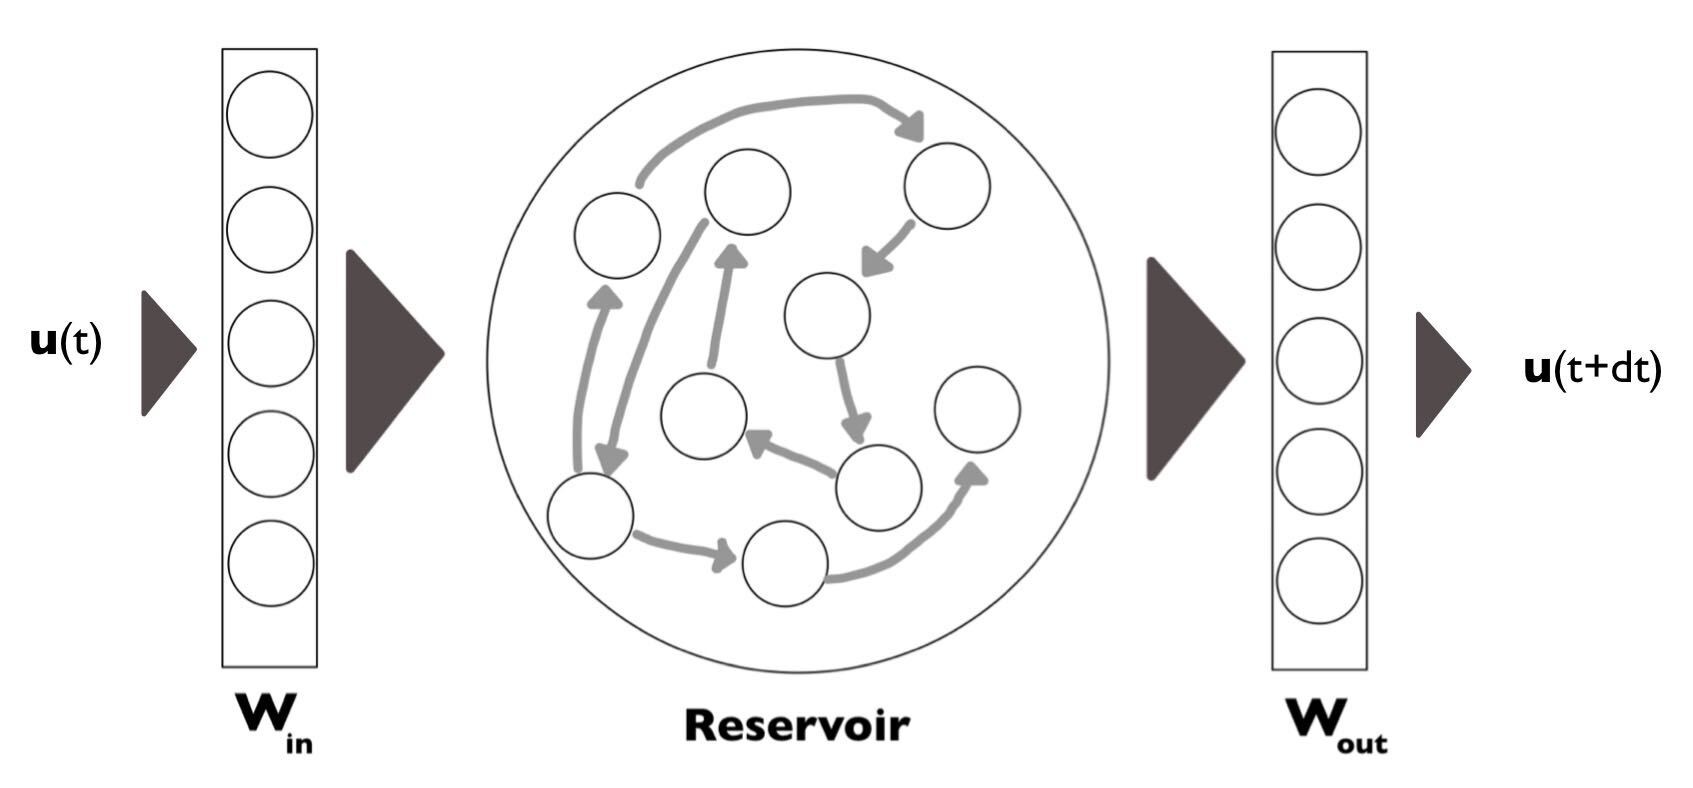
\includegraphics[width=\textwidth]{reservoir_network.jpg}
    \caption{A conceptual diagram of an echo state network. The reservoir is a large sparse matrix with randomly assigned entries \cite{pathak_model-free_2018, lukosevicius_practical_2012}.}
    \label{fig:resnet}
  \end{figure}
\end{frame}

\begin{frame}
  \frametitle{Hyper-parameter Optimization}
  \begin{columns}
    \column[t]{5cm}
      \begin{figure}
        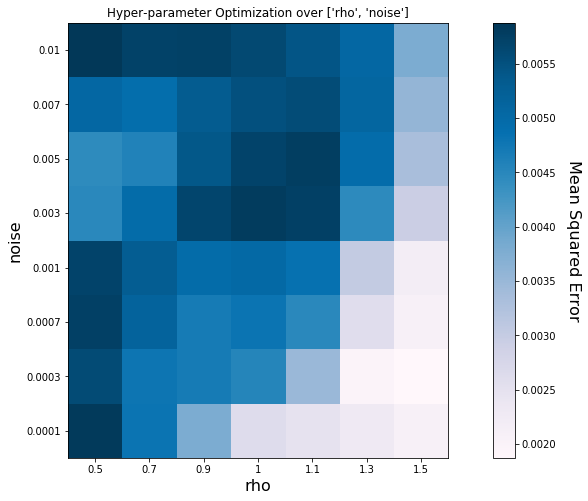
\includegraphics[width=\columnwidth]{solar-angle-gridsearchNP.png}
        \caption{A grid search for the set of noise and spectral radius, $\rho$, that minimizes the mean squared error.}
        \label{fig:gridsearch}
      \end{figure}
    \column[t]{5cm}
      \vspace{1cm}
      \begin{align}
        MSE = \frac{1}{N}\sum_i^N(\hat y - y_i)^2
      \end{align}

      \begin{itemize}
        \item The optimal set of parameters is ``reservoir specific''
        \item Several other parameters need to be optimized such as:
          \begin{itemize}
            \item Reservoir Size
            \item Sparsity
            \item Training Length
          \end{itemize}
      \end{itemize}
  \end{columns}
\end{frame}

\begin{frame}
  \frametitle{Uncertainty Analysis}
  \begin{figure}
    \centering
    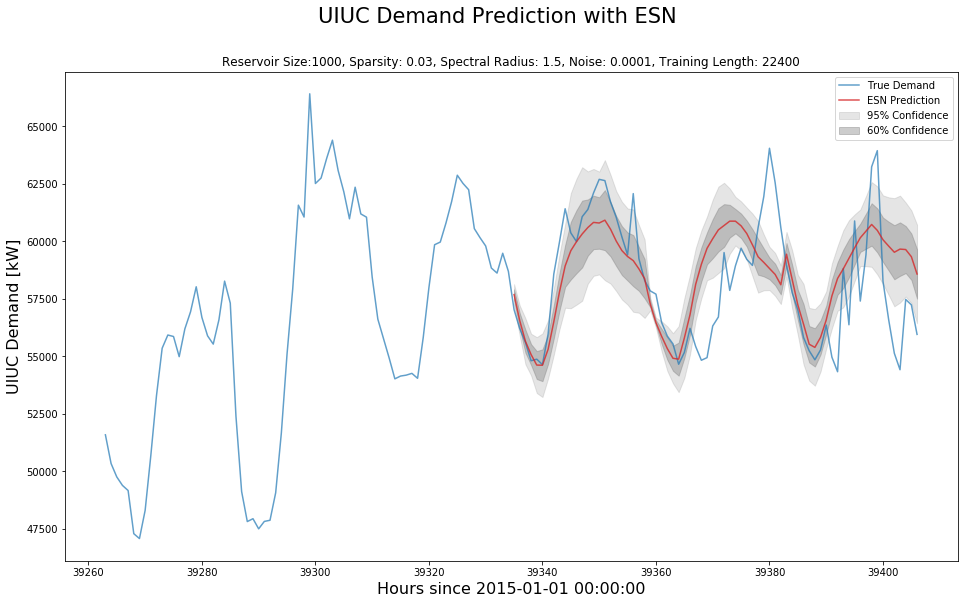
\includegraphics[width=0.85\textwidth]{demsol-bars01.png}
    \caption{Total demand prediction with error bars. The 60\% confidence is $\pm 1\sigma$ and the 95\% confidence interval is $\pm 2\sigma$. Mean is generated from predictions made by several different reservoirs.}
    \label{fig:uncertainty}
  \end{figure}
\end{frame}
